% Template for PLoS
% Version 3.5 March 2018
%
% % % % % % % % % % % % % % % % % % % % % %
%
% -- IMPORTANT NOTE
%
% This template contains comments intended
% to minimize problems and delays during our production
% process. Please follow the template instructions
% whenever possible.
%
% % % % % % % % % % % % % % % % % % % % % % %
%
% Once your paper is accepted for publication,
% PLEASE REMOVE ALL TRACKED CHANGES in this file
% and leave only the final text of your manuscript.
% PLOS recommends the use of latexdiff to track changes during review, as this will help to maintain a clean tex file.
% Visit https://www.ctan.org/pkg/latexdiff?lang=en for info or contact us at latex@plos.org.
%
%
% There are no restrictions on package use within the LaTeX files except that
% no packages listed in the template may be deleted.
%
% Please do not include colors or graphics in the text.
%
% The manuscript LaTeX source should be contained within a single file (do not use \input, \externaldocument, or similar commands).
%
% % % % % % % % % % % % % % % % % % % % % % %
%
% -- FIGURES AND TABLES
%
% Please include tables/figure captions directly after the paragraph where they are first cited in the text.
%
% DO NOT INCLUDE GRAPHICS IN YOUR MANUSCRIPT
% - Figures should be uploaded separately from your manuscript file.
% - Figures generated using LaTeX should be extracted and removed from the PDF before submission.
% - Figures containing multiple panels/subfigures must be combined into one image file before submission.
% For figure citations, please use "Fig" instead of "Figure".
% See http://journals.plos.org/plosone/s/figures for PLOS figure guidelines.
%
% Tables should be cell-based and may not contain:
% - spacing/line breaks within cells to alter layout or alignment
% - do not nest tabular environments (no tabular environments within tabular environments)
% - no graphics or colored text (cell background color/shading OK)
% See http://journals.plos.org/plosone/s/tables for table guidelines.
%
% For tables that exceed the width of the text column, use the adjustwidth environment as illustrated in the example table in text below.
%
% % % % % % % % % % % % % % % % % % % % % % % %
%
% -- EQUATIONS, MATH SYMBOLS, SUBSCRIPTS, AND SUPERSCRIPTS
%
% IMPORTANT
% Below are a few tips to help format your equations and other special characters according to our specifications. For more tips to help reduce the possibility of formatting errors during conversion, please see our LaTeX guidelines at http://journals.plos.org/plosone/s/latex
%
% For inline equations, please be sure to include all portions of an equation in the math environment.
%
% Do not include text that is not math in the math environment.
%
% Please add line breaks to long display equations when possible in order to fit size of the column.
%
% For inline equations, please do not include punctuation (commas, etc) within the math environment unless this is part of the equation.
%
% When adding superscript or subscripts outside of brackets/braces, please group using {}.
%
% Do not use \cal for caligraphic font.  Instead, use \mathcal{}
%
% % % % % % % % % % % % % % % % % % % % % % % %
%
% Please contact latex@plos.org with any questions.
%
% % % % % % % % % % % % % % % % % % % % % % % %

\documentclass[10pt,letterpaper]{article}
\usepackage[top=0.85in,left=2.75in,footskip=0.75in]{geometry}

% amsmath and amssymb packages, useful for mathematical formulas and symbols
\usepackage{amsmath,amssymb}

% Use adjustwidth environment to exceed column width (see example table in text)
\usepackage{changepage}

% Use Unicode characters when possible
\usepackage[utf8x]{inputenc}

% textcomp package and marvosym package for additional characters
\usepackage{textcomp,marvosym}

% cite package, to clean up citations in the main text. Do not remove.
% \usepackage{cite}

% Use nameref to cite supporting information files (see Supporting Information section for more info)
\usepackage{nameref,hyperref}

% line numbers
\usepackage[right]{lineno}

% ligatures disabled
\usepackage{microtype}
\DisableLigatures[f]{encoding = *, family = * }

% color can be used to apply background shading to table cells only
\usepackage[table]{xcolor}

% array package and thick rules for tables
\usepackage{array}

% create "+" rule type for thick vertical lines
\newcolumntype{+}{!{\vrule width 2pt}}

% create \thickcline for thick horizontal lines of variable length
\newlength\savedwidth
\newcommand\thickcline[1]{%
  \noalign{\global\savedwidth\arrayrulewidth\global\arrayrulewidth 2pt}%
  \cline{#1}%
  \noalign{\vskip\arrayrulewidth}%
  \noalign{\global\arrayrulewidth\savedwidth}%
}

% \thickhline command for thick horizontal lines that span the table
\newcommand\thickhline{\noalign{\global\savedwidth\arrayrulewidth\global\arrayrulewidth 2pt}%
\hline
\noalign{\global\arrayrulewidth\savedwidth}}


% Remove comment for double spacing
%\usepackage{setspace}
%\doublespacing

% Text layout
\raggedright
\setlength{\parindent}{0.5cm}
\textwidth 5.25in
\textheight 8.75in

% Bold the 'Figure #' in the caption and separate it from the title/caption with a period
% Captions will be left justified
\usepackage[aboveskip=1pt,labelfont=bf,labelsep=period,justification=raggedright,singlelinecheck=off]{caption}
\renewcommand{\figurename}{Fig}

% Use the PLoS provided BiBTeX style
% \bibliographystyle{plos2015}

% Remove brackets from numbering in List of References
\makeatletter
\renewcommand{\@biblabel}[1]{\quad#1.}
\makeatother



% Header and Footer with logo
\usepackage{lastpage,fancyhdr,graphicx}
\usepackage{epstopdf}
%\pagestyle{myheadings}
\pagestyle{fancy}
\fancyhf{}
%\setlength{\headheight}{27.023pt}
%\lhead{
\includegraphics[width=2.0in]{PLOS-submission.eps}}
\rfoot{\thepage/\pageref{LastPage}}
\renewcommand{\headrulewidth}{0pt}
\renewcommand{\footrule}{\hrule height 2pt \vspace{2mm}}
\fancyheadoffset[L]{2.25in}
\fancyfootoffset[L]{2.25in}
\lfoot{\today}

%% Include all macros below

\newcommand{\lorem}{{\bf LOREM}}
\newcommand{\ipsum}{{\bf IPSUM}}


% Pandoc citation processing

\usepackage{booktabs}
\usepackage{longtable}
\usepackage{array}
\usepackage{multirow}
\usepackage{wrapfig}
\usepackage{float}
\usepackage{colortbl}
\usepackage{pdflscape}
\usepackage{tabu}
\usepackage{threeparttable}
\usepackage{threeparttablex}
\usepackage[normalem]{ulem}
\usepackage{makecell}
\usepackage{xcolor}



\usepackage{forarray}
\usepackage{xstring}
\newcommand{\getIndex}[2]{
  \ForEach{,}{\IfEq{#1}{\thislevelitem}{\number\thislevelcount\ExitForEach}{}}{#2}
}

\setcounter{secnumdepth}{0}

\newcommand{\getAff}[1]{
  \getIndex{#1}{Some Institute of Technology,Another University}
}

\providecommand{\tightlist}{%
  \setlength{\itemsep}{0pt}\setlength{\parskip}{0pt}}

\begin{document}
\vspace*{0.2in}

% Title must be 250 characters or less.
\begin{flushleft}
{\Large
\textbf\newline{Short-term real-time prediction of total number of reported COVID-19
cases in South Africa - A Bayesian Temporal Modeling Approch} % Please use "sentence case" for title and headings (capitalize only the first word in a title (or heading), the first word in a subtitle (or subheading), and any proper nouns).
}
\newline
% Insert author names, affiliations and corresponding author email (do not include titles, positions, or degrees).
\\
Belay Birlie Yimer\textsuperscript{\getAff{University of Manchester, Uk;}, \getAff{Hasselt University, Belgium.}}\textsuperscript{*},
Ziv Shkedy\textsuperscript{\getAff{Hasselt University}}\\
\bigskip
\textbf{\getAff{Some Institute of Technology}}Department 1, Street, City, State, Zip\\
\textbf{\getAff{Another University}}Department 2, Street, City, State, Zip\\
\bigskip
* Corresponding author: belaybirlie.yimer@manchester.ac.uk\\
\end{flushleft}
% Please keep the abstract below 300 words
\section*{Abstract}
To be updated.

% Please keep the Author Summary between 150 and 200 words
% Use first person. PLOS ONE authors please skip this step.
% Author Summary not valid for PLOS ONE submissions.
\section*{Author summary}
To be updated.

\linenumbers

% Use "Eq" instead of "Equation" for equation citations.
\hypertarget{introduction}{%
\section{Introduction}\label{introduction}}

To be updated Here are two sample references: {[}1,2{]}.

\hypertarget{methods}{%
\section{Methods}\label{methods}}

\hypertarget{data}{%
\subsection{Data}\label{data}}

We downloaded data from Coronavirus COVID-19 (2019-nCoV) Data Repository
for South Africa maintained by Data Science for Social Impact research
group at the University of Pretoria {[}ref{]}. The data repository
captures the daily number of new cases, number of tests, number of
deaths and recoveries. Our primary outcome of interest was the daily
number of newly diagnosed COVID-19 cases and the unit of time used in
modelling was a day. We used the daily case reports from March 12, 2020,
until February 15, 2021, in our analysis.

\hypertarget{statistical-analysis}{%
\subsection{Statistical analysis}\label{statistical-analysis}}

We considered two widely used temporal models to model the daily number
of newly diagnosed COVID-19 cases. We let \(Y(t)\) denote the daily
number of newly diagnosed COVID-19 cases at time \(t\) and \(\mu(t)\)
represent the expected number of cases at time \(t\). We considered a
Negative binomial distribution for \(Y(t)\) to account for possible
overdispersion. That is, \(Y(t) \sim NB(\mu(t), \delta)\), where
\(\delta\) is the overdispersion parameter. We considered two temporal
models to capture the trend over time: a random walk of order one
(\(RW(1)\)) and an autoregressive model of order one (\(AR(1)\))
{[}ref{]}. The two models were chosen becuse

The \(AR(1)\) model {[}ref{]} is given by,

\[
\begin{aligned}
 Y(t) &\sim NB(\mu(t), \delta) \ \ t=1, \dots, n,\\
 log(\mu(t)) &= \alpha+u_t, \\
 u_1 &\sim N(0, \tau_u(1-\rho^2)^{-1}),  \\
  u_t &=\rho u_{t-1} +\epsilon_t, \ \ t=2, \dots, n,  \\
  \epsilon_t & \sim N(0, \tau_{\epsilon}),
\end{aligned}
\] where, \(\alpha\) is an intercept, \(\rho\) a temporal correlation
term (with \(|\rho|<1\)) and \(\epsilon_t\) is a Gaussian error term
with zero mean and precision \(\tau_u\).

Similarly, the \(RW(1)\) model {[}ref{]} is given by, \[
\begin{aligned}
 Y(t) &\sim NB(\mu(t), \delta) \ \ t=1, \dots, n,\\
 log(\mu(t)) &= \alpha+u_t, \\
 u_t-u_{t-1} &\sim N(0, \tau_u), \ \ t=2, \dots, n,
\end{aligned}
\] where \(\alpha\) is the intercept term as before and \(\tau_u\) is
the precison parameter.

The two models were fitted within the Bayesian framework using
\emph{inla} {[}ref{]}. To complete the specification of both models, we
assume the following priors. For the \(AR(1)\) model, we denote
\(\theta_1=log(\tau_u(1-\rho^2))\) where \(\Gamma(10,100)\) prior is
specified for \(\theta_1\), and we denote
\(\theta_2=log\frac{1+\rho}{1-\rho}\) and assume a \(N(0, 0.15)\) prior
for \(\theta\). Similarly, we represent the precison parameter of
\(RW(1)\), \(\tau_u\), as \(\theta=log(\tau_u)\) and assume a
\(\Gamma (10,100)\) prior for \(\theta\). To assess the models' accuracy
in predicting cases, we present the forecast period's actual observed
values and the predicted values.Additionally, the model fits were
evaluated by using DIC (Deviance information criteria). The computer
code that we used for our analyses is avaliable at
https://github.com/belayb/COVIDincidenceSA.

\hypertarget{results}{%
\section{Results}\label{results}}

Figure 1 (Top panel) presents the daily number of reported COVID-19
cases from 5 March 2020 to 15 February 2021. Similar to elsewhere in the
world, South Africa pass through a two-wave pandemic. The first peak of
the epidemic was on ----, followed by a second peak in January 2021.
Figure 1 (Bottom Panel) presents the cumulative number of new reported
COVID-19 cases and tests performed. To date, 1,353,176 tests have been
conducted, corresponding to a testing rate of 22.816 per 1000
population. There was a significant correlation between the number of
cases detected and the number of tests performed daily (Rho = 0.7759,
p-value\textless{} 0.001).

\begin{figure}
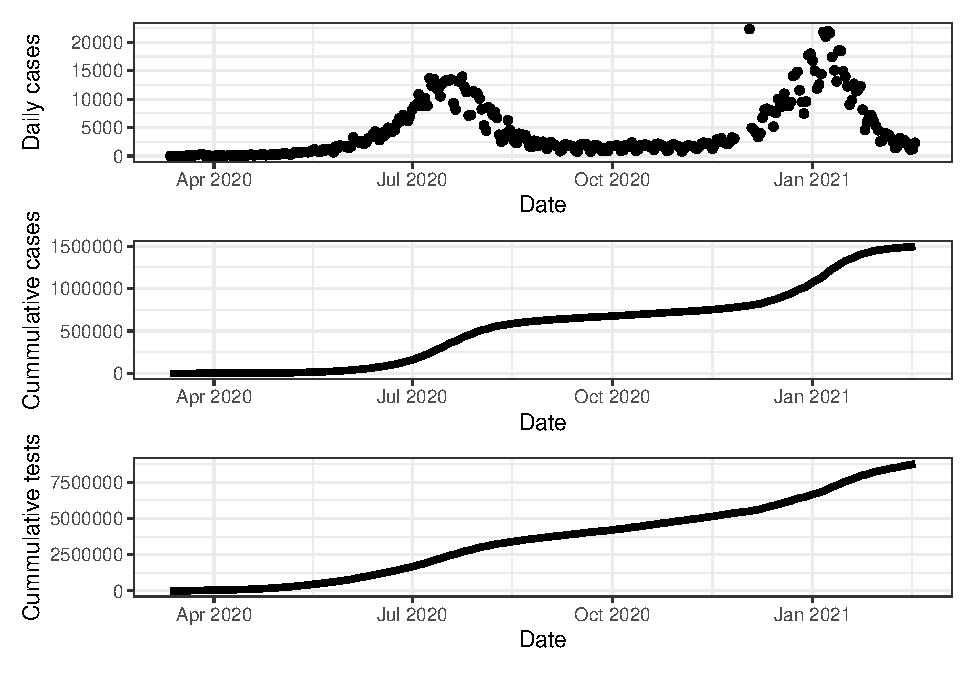
\includegraphics[width=0.99\linewidth]{COVIDincidenceSA_files/figure-latex/unnamed-chunk-4-1} \caption{Daily new COVID-19 cases.}\label{fig:unnamed-chunk-4}
\end{figure}

\begin{figure}
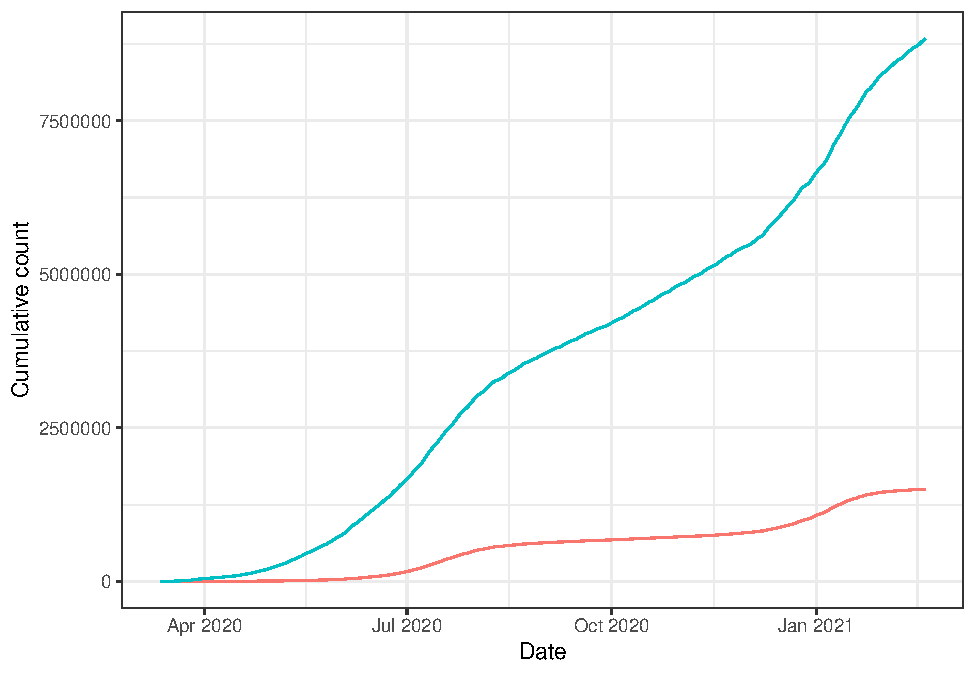
\includegraphics[width=0.99\linewidth]{COVIDincidenceSA_files/figure-latex/unnamed-chunk-5-1} \caption{cummulative cases and cummulative tests.}\label{fig:unnamed-chunk-5}
\end{figure}

\hypertarget{short-term-prediction-of-the-total-number-of-reported-covid-19-cases}{%
\subsection{Short-term prediction of the total number of reported
COVID-19
cases}\label{short-term-prediction-of-the-total-number-of-reported-covid-19-cases}}

The models described in the previous section were all considered for
modeling cumulative cases.The parameter estimates for the different
models are presented in Supplementary Table 1. As mentioned in the
previous section, our main interest is to produce a short term forecast
for the number of reported cases and deaths. As depicted from the
short-term forecasts for the three models fitted to cases (see Fig. 5,
Table 2), all three models appear to fit the observed data (within the
estimation period) well with the 3 parameter and 4 parameter logistic
models providing very similar predictions over the 30-day ahead period.

\begin{figure}
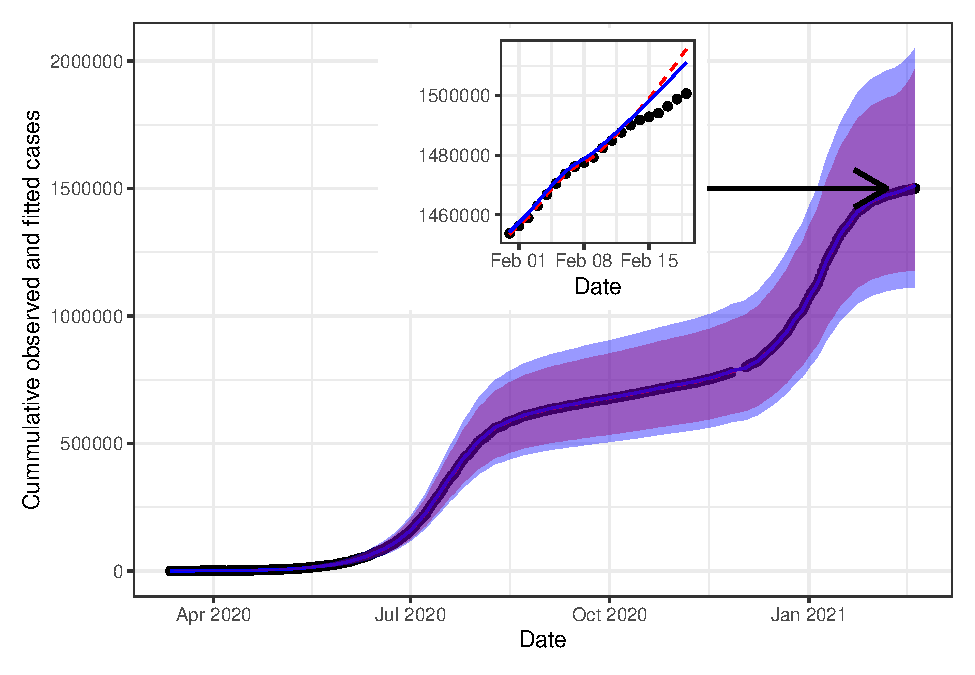
\includegraphics[width=0.99\linewidth]{COVIDincidenceSA_files/figure-latex/unnamed-chunk-9-1} \caption{Fitted and observed data}\label{fig:unnamed-chunk-9}
\end{figure}

\begin{table}

\caption{\label{tab:unnamed-chunk-10}Short-term predictions of total number of reported cases at the national level under the RW1 model. Estimation period 05/03/2020-08/02/2021}
\centering
\begin{tabular}[t]{l|l|r|r|l}
\hline
  & Date & Total & Prediction & Prediction Interval\\
\hline
329 & 2021-02-11 & 1484900 & 1485425 & (1172933.36-1870556.26)\\
\hline
330 & 2021-02-12 & 1487681 & 1488625 & (1174169.39-1877507.47)\\
\hline
331 & 2021-02-13 & 1490063 & 1491972 & (1175202.53-1885836.24)\\
\hline
332 & 2021-02-14 & 1491807 & 1495472 & (1176089.35-1895548.55)\\
\hline
333 & 2021-02-15 & 1492909 & 1499134 & (1176864-1906676.65)\\
\hline
334 & 2021-02-16 & 1494119 & 1502964 & (1177549.26-1919266.52)\\
\hline
335 & 2021-02-17 & 1496439 & 1506970 & (1178161.06-1933372.71)\\
\hline
336 & 2021-02-18 & 1498766 & 1511162 & (1178711.39-1949056.38)\\
\hline
337 & 2021-02-19 & 1500677 & 1515548 & (1179209.55-1966383.94)\\
\hline
\end{tabular}
\end{table}

\begin{table}

\caption{\label{tab:unnamed-chunk-10}Short-term predictions of total number of reported cases at the national level under the AR1 model. Estimation period 05/03/2020-08/02/2021}
\centering
\begin{tabular}[t]{l|l|r|r|l}
\hline
  & Date & Total & Prediction & Prediction Interval\\
\hline
329 & 2021-02-11 & 1484900 & 1486312 & (1107420.98-1978162.82)\\
\hline
330 & 2021-02-12 & 1487681 & 1489173 & (1108639.61-1983981.29)\\
\hline
331 & 2021-02-13 & 1490063 & 1492102 & (1109681.58-1990659.34)\\
\hline
332 & 2021-02-14 & 1491807 & 1495099 & (1110591.96-1998160.29)\\
\hline
333 & 2021-02-15 & 1492909 & 1498166 & (1111398.75-2006463.55)\\
\hline
334 & 2021-02-16 & 1494119 & 1501303 & (1112121.57-2015558.08)\\
\hline
335 & 2021-02-17 & 1496439 & 1504510 & (1112774.74-2025437.2)\\
\hline
336 & 2021-02-18 & 1498766 & 1507790 & (1113369.03-2036097.59)\\
\hline
337 & 2021-02-19 & 1500677 & 1511143 & (1113912.84-2047538.12)\\
\hline
\end{tabular}
\end{table}

\hypertarget{references}{%
\section*{References}\label{references}}
\addcontentsline{toc}{section}{References}

\hypertarget{refs}{}
\leavevmode\hypertarget{ref-Feynman1963118}{}%
1. Feynman RP, Vernon Jr. FL. The theory of a general quantum system
interacting with a linear dissipative system. Annals of Physics.
1963;24: 118--173.
doi:\href{https://doi.org/10.1016/0003-4916(63)90068-X}{10.1016/0003-4916(63)90068-X}

\leavevmode\hypertarget{ref-Dirac1953888}{}%
2. Dirac PA. The lorentz transformation and absolute time. Physica.
1953;19: 888--896.
doi:\href{https://doi.org/10.1016/S0031-8914(53)80099-6}{10.1016/S0031-8914(53)80099-6}

\nolinenumbers


\end{document}

